\documentclass[a4paper]{book}
\usepackage{a4wide}
\usepackage{makeidx}
\usepackage{graphicx}
\usepackage{multicol}
\usepackage{float}
\usepackage{listings}
\usepackage{color}
\usepackage{textcomp}
\usepackage{alltt}
\usepackage{times}
\usepackage{ifpdf}
\ifpdf
\usepackage[pdftex,
            pagebackref=true,
            colorlinks=true,
            linkcolor=blue,
            unicode
           ]{hyperref}
\else
\usepackage[ps2pdf,
            pagebackref=true,
            colorlinks=true,
            linkcolor=blue,
            unicode
           ]{hyperref}
\usepackage{pspicture}
\fi
\usepackage[utf8]{inputenc}
\usepackage{doxygen}
\lstset{language=C++,inputencoding=utf8,basicstyle=\footnotesize,breaklines=true,breakatwhitespace=true,tabsize=8,numbers=left }
\makeindex
\setcounter{tocdepth}{3}
\renewcommand{\footrulewidth}{0.4pt}
\begin{document}
\hypersetup{pageanchor=false}
\begin{titlepage}
\vspace*{7cm}
\begin{center}
{\Large Reference Manual}\\
\vspace*{1cm}
{\large Generated by Doxygen 1.6.3}\\
\vspace*{0.5cm}
{\small Wed Feb 1 00:24:43 2012}\\
\end{center}
\end{titlepage}
\clearemptydoublepage
\pagenumbering{roman}
\tableofcontents
\clearemptydoublepage
\pagenumbering{arabic}
\hypersetup{pageanchor=true}
\chapter{Class Index}
\section{Class List}
Here are the classes, structs, unions and interfaces with brief descriptions:\begin{DoxyCompactList}
\item\contentsline{section}{\hyperlink{structcgpa}{cgpa} }{\pageref{structcgpa}}{}
\item\contentsline{section}{\hyperlink{structchoice}{choice} }{\pageref{structchoice}}{}
\end{DoxyCompactList}

\chapter{File Index}
\section{File List}
Here is a list of all files with brief descriptions:\begin{DoxyCompactList}
\item\contentsline{section}{code/\hyperlink{allocation_8c}{allocation.c} }{\pageref{allocation_8c}}{}
\end{DoxyCompactList}

\chapter{Class Documentation}
\hypertarget{structnode}{
\section{node Struct Reference}
\label{structnode}\index{node@{node}}
}


Collaboration diagram for node:\nopagebreak
\begin{figure}[H]
\begin{center}
\leavevmode
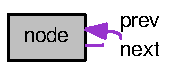
\includegraphics[width=117pt]{structnode__coll__graph}
\end{center}
\end{figure}
\subsection*{Public Attributes}
\begin{DoxyCompactItemize}
\item 
struct \hyperlink{structnode}{node} $\ast$ \hyperlink{structnode_a23dd2ff244acbbf20ec4408f81d76d9c}{prev}
\item 
struct \hyperlink{structnode}{node} $\ast$ \hyperlink{structnode_ad465c36cd29be2935f9e1bee1a3eaa03}{next}
\item 
char \hyperlink{structnode_af67fef838619da259b5c424c8fe5f718}{name} \mbox{[}NAME\_\-SIZE\mbox{]}
\item 
int \hyperlink{structnode_a972b8b8be90e29c40676be5d34ad3b1d}{first}
\item 
int \hyperlink{structnode_ae9b51f363ea789f5f6ec2fbc0b2a8086}{third}
\end{DoxyCompactItemize}


\subsection{Detailed Description}


Definition at line 35 of file cardtrick.c.



\subsection{Member Data Documentation}
\hypertarget{structnode_a972b8b8be90e29c40676be5d34ad3b1d}{
\index{node@{node}!first@{first}}
\index{first@{first}!node@{node}}
\subsubsection[{first}]{\setlength{\rightskip}{0pt plus 5cm}int {\bf node.first}}}
\label{structnode_a972b8b8be90e29c40676be5d34ad3b1d}
No of letters in first word 

Definition at line 43 of file cardtrick.c.

\hypertarget{structnode_af67fef838619da259b5c424c8fe5f718}{
\index{node@{node}!name@{name}}
\index{name@{name}!node@{node}}
\subsubsection[{name}]{\setlength{\rightskip}{0pt plus 5cm}char {\bf node.name}\mbox{[}NAME\_\-SIZE\mbox{]}}}
\label{structnode_af67fef838619da259b5c424c8fe5f718}
Node Data: Name of Card 

Definition at line 41 of file cardtrick.c.

\hypertarget{structnode_ad465c36cd29be2935f9e1bee1a3eaa03}{
\index{node@{node}!next@{next}}
\index{next@{next}!node@{node}}
\subsubsection[{next}]{\setlength{\rightskip}{0pt plus 5cm}struct {\bf node}$\ast$ {\bf node.next}}}
\label{structnode_ad465c36cd29be2935f9e1bee1a3eaa03}
Next pointer for doubly linked node 

Definition at line 39 of file cardtrick.c.

\hypertarget{structnode_a23dd2ff244acbbf20ec4408f81d76d9c}{
\index{node@{node}!prev@{prev}}
\index{prev@{prev}!node@{node}}
\subsubsection[{prev}]{\setlength{\rightskip}{0pt plus 5cm}struct {\bf node}$\ast$ {\bf node.prev}}}
\label{structnode_a23dd2ff244acbbf20ec4408f81d76d9c}
Previous pointer for doubly linked node 

Definition at line 37 of file cardtrick.c.

\hypertarget{structnode_ae9b51f363ea789f5f6ec2fbc0b2a8086}{
\index{node@{node}!third@{third}}
\index{third@{third}!node@{node}}
\subsubsection[{third}]{\setlength{\rightskip}{0pt plus 5cm}int {\bf node.third}}}
\label{structnode_ae9b51f363ea789f5f6ec2fbc0b2a8086}
No of letters in third word 

Definition at line 45 of file cardtrick.c.



The documentation for this struct was generated from the following file:\begin{DoxyCompactItemize}
\item 
code/\hyperlink{cardtrick_8c}{cardtrick.c}\end{DoxyCompactItemize}

\hypertarget{structqueue}{
\section{queue Struct Reference}
\label{structqueue}\index{queue@{queue}}
}


Collaboration diagram for queue:\nopagebreak
\begin{figure}[H]
\begin{center}
\leavevmode
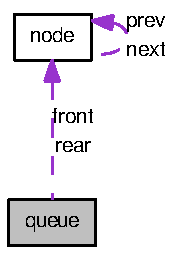
\includegraphics[width=120pt]{structqueue__coll__graph}
\end{center}
\end{figure}
\subsection*{Public Attributes}
\begin{DoxyCompactItemize}
\item 
struct \hyperlink{structnode}{node} $\ast$ \hyperlink{structqueue_a2798de43b9b1439dbbef5dfd7bb78d8e}{front}
\item 
struct \hyperlink{structnode}{node} $\ast$ \hyperlink{structqueue_aa5381eaa02a38f052e2d0fdf59849af3}{rear}
\end{DoxyCompactItemize}


\subsection{Detailed Description}


Definition at line 48 of file cardtrick.c.



\subsection{Member Data Documentation}
\hypertarget{structqueue_a2798de43b9b1439dbbef5dfd7bb78d8e}{
\index{queue@{queue}!front@{front}}
\index{front@{front}!queue@{queue}}
\subsubsection[{front}]{\setlength{\rightskip}{0pt plus 5cm}struct {\bf node}$\ast$ {\bf queue.front}}}
\label{structqueue_a2798de43b9b1439dbbef5dfd7bb78d8e}
Front pointer of queue: A node will always be removed from front 

Definition at line 53 of file cardtrick.c.

\hypertarget{structqueue_aa5381eaa02a38f052e2d0fdf59849af3}{
\index{queue@{queue}!rear@{rear}}
\index{rear@{rear}!queue@{queue}}
\subsubsection[{rear}]{\setlength{\rightskip}{0pt plus 5cm}struct {\bf node}$\ast$ {\bf queue.rear}}}
\label{structqueue_aa5381eaa02a38f052e2d0fdf59849af3}
Rear pointer of queue: A node will always be inserted to the rear 

Definition at line 58 of file cardtrick.c.



The documentation for this struct was generated from the following file:\begin{DoxyCompactItemize}
\item 
code/\hyperlink{cardtrick_8c}{cardtrick.c}\end{DoxyCompactItemize}

\hypertarget{structstack}{
\section{stack Struct Reference}
\label{structstack}\index{stack@{stack}}
}


Collaboration diagram for stack:\nopagebreak
\begin{figure}[H]
\begin{center}
\leavevmode
\includegraphics[width=119pt]{structstack__coll__graph}
\end{center}
\end{figure}
\subsection*{Public Attributes}
\begin{DoxyCompactItemize}
\item 
struct \hyperlink{structnode}{node} $\ast$ \hyperlink{structstack_ab1713a4aa13c94c6676f0ed3f33478dc}{top}
\end{DoxyCompactItemize}


\subsection{Detailed Description}


Definition at line 61 of file cardtrick.c.



\subsection{Member Data Documentation}
\hypertarget{structstack_ab1713a4aa13c94c6676f0ed3f33478dc}{
\index{stack@{stack}!top@{top}}
\index{top@{top}!stack@{stack}}
\subsubsection[{top}]{\setlength{\rightskip}{0pt plus 5cm}struct {\bf node}$\ast$ {\bf stack.top}}}
\label{structstack_ab1713a4aa13c94c6676f0ed3f33478dc}
Top pointer of stack: A node will always be pushed and popped at the top. 

Definition at line 66 of file cardtrick.c.



The documentation for this struct was generated from the following file:\begin{DoxyCompactItemize}
\item 
code/\hyperlink{cardtrick_8c}{cardtrick.c}\end{DoxyCompactItemize}

\chapter{File Documentation}
\hypertarget{cardtrick_8c}{
\section{code/cardtrick.c File Reference}
\label{cardtrick_8c}\index{code/cardtrick.c@{code/cardtrick.c}}
}
{\ttfamily \#include $<$errno.h$>$}\par
{\ttfamily \#include $<$getopt.h$>$}\par
{\ttfamily \#include $<$stdio.h$>$}\par
{\ttfamily \#include $<$stdlib.h$>$}\par
{\ttfamily \#include $<$string.h$>$}\par
Include dependency graph for cardtrick.c:\nopagebreak
\begin{figure}[H]
\begin{center}
\leavevmode
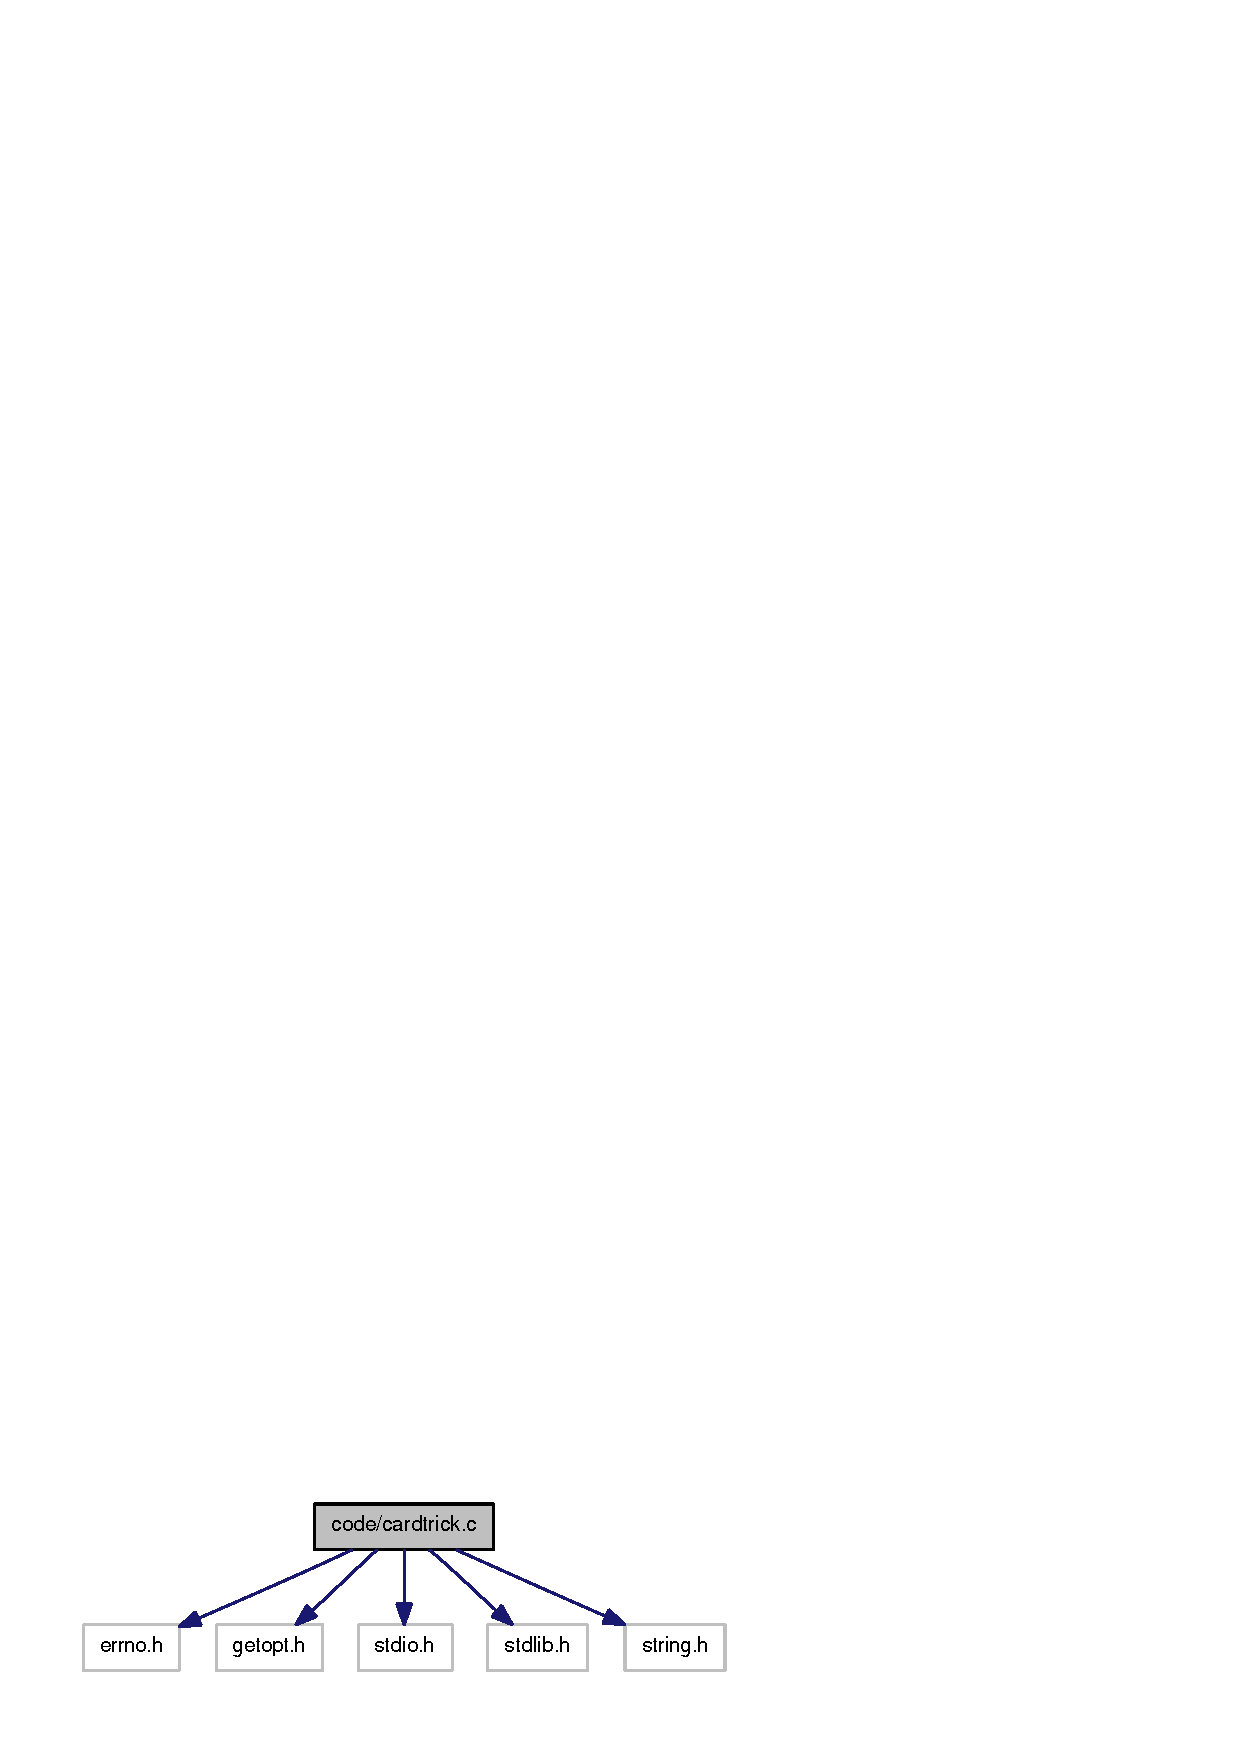
\includegraphics[width=176pt]{cardtrick_8c__incl}
\end{center}
\end{figure}
\subsection*{Classes}
\begin{DoxyCompactItemize}
\item 
struct \hyperlink{structnode}{node}
\item 
struct \hyperlink{structqueue}{queue}
\item 
struct \hyperlink{structstack}{stack}
\end{DoxyCompactItemize}
\subsection*{Defines}
\begin{DoxyCompactItemize}
\item 
\#define \hyperlink{cardtrick_8c_a76ebf98e05f78e90288d56fb4caf1280}{pr\_\-info}(args...)~fprintf(stdout, \#\#args)
\item 
\#define \hyperlink{cardtrick_8c_ab7f9743ece3b8b02877758771a177c7c}{pr\_\-err}(args...)~fprintf(stdout, \#\#args)
\item 
\#define \hyperlink{cardtrick_8c_a46ff2bfbf0d44b8466a2251d5bd5e6f8}{NOMEM}~\char`\"{}No memory available$\backslash$n\char`\"{}
\item 
\#define \hyperlink{cardtrick_8c_af7a8f58fd33bff0a1ccc65fcfbfbc8b4}{CHINVAL}~\char`\"{}Not a valid choice$\backslash$n\char`\"{}
\item 
\#define \hyperlink{cardtrick_8c_a834e9a379307f869a10f4da078be5786}{NAME\_\-SIZE}~3
\item 
\#define \hyperlink{cardtrick_8c_a206b6f5362e56b51ca957635350b70b6}{ONE}~\char`\"{}One\char`\"{}
\item 
\#define \hyperlink{cardtrick_8c_a888e15353eb3d330c743dbdeb47117e2}{TWO}~\char`\"{}Two\char`\"{}
\item 
\#define \hyperlink{cardtrick_8c_a1859c475c0bde19dfc1101e35d71b939}{THREE}~\char`\"{}Three\char`\"{}
\item 
\#define \hyperlink{cardtrick_8c_a64a9b58c6a5bcd3724f3b56ad6d006a7}{FOUR}~\char`\"{}Four\char`\"{}
\item 
\#define \hyperlink{cardtrick_8c_a18ced145d1fdc806b5006bd4c2857026}{FIVE}~\char`\"{}Five\char`\"{}
\item 
\#define \hyperlink{cardtrick_8c_afad3d8b3d66fceadb1732af784734c75}{SIX}~\char`\"{}Six\char`\"{}
\item 
\#define \hyperlink{cardtrick_8c_ac537e6e7dad3ecef73fc3fc4f14fe020}{SEVEN}~\char`\"{}Seven\char`\"{}
\item 
\#define \hyperlink{cardtrick_8c_aaf6cfeda610d5092df7deb18fd5d63c2}{EIGHT}~\char`\"{}Eight\char`\"{}
\item 
\#define \hyperlink{cardtrick_8c_aef08329d0c1db97d7b269330ae9a70af}{NINE}~\char`\"{}Nine\char`\"{}
\item 
\#define \hyperlink{cardtrick_8c_aabc53aa7e6353d8f58b8ae93fd015fab}{TEN}~\char`\"{}Ten\char`\"{}
\item 
\#define \hyperlink{cardtrick_8c_aa941833decb7feaf364825bca39896b7}{JACK}~\char`\"{}Jack\char`\"{}
\item 
\#define \hyperlink{cardtrick_8c_a64648880b0877cbf45dd176839aff27e}{QUEEN}~\char`\"{}Queen\char`\"{}
\item 
\#define \hyperlink{cardtrick_8c_a4053d9a782c54549f5faf06c3c95262b}{KING}~\char`\"{}King\char`\"{}
\item 
\#define \hyperlink{cardtrick_8c_aa5c6b846f4b3de021da5d2873667bbba}{HEARTS}~\char`\"{}Hearts\char`\"{}
\item 
\#define \hyperlink{cardtrick_8c_a76648664c0dd95e4fc8fd2e8b886ff6b}{DIAMONDS}~\char`\"{}Diamonds\char`\"{}
\item 
\#define \hyperlink{cardtrick_8c_a1a956774e7c7633cfe6a47a8f0af772e}{SPADES}~\char`\"{}Spades\char`\"{}
\item 
\#define \hyperlink{cardtrick_8c_ab701fc080416630326132e29bce2f419}{CLUBS}~\char`\"{}Clubs\char`\"{}
\end{DoxyCompactItemize}
\subsection*{Functions}
\begin{DoxyCompactItemize}
\item 
int \hyperlink{cardtrick_8c_a3c04138a5bfe5d72780bb7e82a18e627}{main} (int argc, char $\ast$$\ast$argv)
\end{DoxyCompactItemize}


\subsection{Define Documentation}
\hypertarget{cardtrick_8c_af7a8f58fd33bff0a1ccc65fcfbfbc8b4}{
\index{cardtrick.c@{cardtrick.c}!CHINVAL@{CHINVAL}}
\index{CHINVAL@{CHINVAL}!cardtrick.c@{cardtrick.c}}
\subsubsection[{CHINVAL}]{\setlength{\rightskip}{0pt plus 5cm}\#define CHINVAL~\char`\"{}Not a valid choice$\backslash$n\char`\"{}}}
\label{cardtrick_8c_af7a8f58fd33bff0a1ccc65fcfbfbc8b4}


Definition at line 15 of file cardtrick.c.

\hypertarget{cardtrick_8c_ab701fc080416630326132e29bce2f419}{
\index{cardtrick.c@{cardtrick.c}!CLUBS@{CLUBS}}
\index{CLUBS@{CLUBS}!cardtrick.c@{cardtrick.c}}
\subsubsection[{CLUBS}]{\setlength{\rightskip}{0pt plus 5cm}\#define CLUBS~\char`\"{}Clubs\char`\"{}}}
\label{cardtrick_8c_ab701fc080416630326132e29bce2f419}


Definition at line 33 of file cardtrick.c.

\hypertarget{cardtrick_8c_a76648664c0dd95e4fc8fd2e8b886ff6b}{
\index{cardtrick.c@{cardtrick.c}!DIAMONDS@{DIAMONDS}}
\index{DIAMONDS@{DIAMONDS}!cardtrick.c@{cardtrick.c}}
\subsubsection[{DIAMONDS}]{\setlength{\rightskip}{0pt plus 5cm}\#define DIAMONDS~\char`\"{}Diamonds\char`\"{}}}
\label{cardtrick_8c_a76648664c0dd95e4fc8fd2e8b886ff6b}


Definition at line 31 of file cardtrick.c.

\hypertarget{cardtrick_8c_aaf6cfeda610d5092df7deb18fd5d63c2}{
\index{cardtrick.c@{cardtrick.c}!EIGHT@{EIGHT}}
\index{EIGHT@{EIGHT}!cardtrick.c@{cardtrick.c}}
\subsubsection[{EIGHT}]{\setlength{\rightskip}{0pt plus 5cm}\#define EIGHT~\char`\"{}Eight\char`\"{}}}
\label{cardtrick_8c_aaf6cfeda610d5092df7deb18fd5d63c2}


Definition at line 24 of file cardtrick.c.

\hypertarget{cardtrick_8c_a18ced145d1fdc806b5006bd4c2857026}{
\index{cardtrick.c@{cardtrick.c}!FIVE@{FIVE}}
\index{FIVE@{FIVE}!cardtrick.c@{cardtrick.c}}
\subsubsection[{FIVE}]{\setlength{\rightskip}{0pt plus 5cm}\#define FIVE~\char`\"{}Five\char`\"{}}}
\label{cardtrick_8c_a18ced145d1fdc806b5006bd4c2857026}


Definition at line 21 of file cardtrick.c.

\hypertarget{cardtrick_8c_a64a9b58c6a5bcd3724f3b56ad6d006a7}{
\index{cardtrick.c@{cardtrick.c}!FOUR@{FOUR}}
\index{FOUR@{FOUR}!cardtrick.c@{cardtrick.c}}
\subsubsection[{FOUR}]{\setlength{\rightskip}{0pt plus 5cm}\#define FOUR~\char`\"{}Four\char`\"{}}}
\label{cardtrick_8c_a64a9b58c6a5bcd3724f3b56ad6d006a7}


Definition at line 20 of file cardtrick.c.

\hypertarget{cardtrick_8c_aa5c6b846f4b3de021da5d2873667bbba}{
\index{cardtrick.c@{cardtrick.c}!HEARTS@{HEARTS}}
\index{HEARTS@{HEARTS}!cardtrick.c@{cardtrick.c}}
\subsubsection[{HEARTS}]{\setlength{\rightskip}{0pt plus 5cm}\#define HEARTS~\char`\"{}Hearts\char`\"{}}}
\label{cardtrick_8c_aa5c6b846f4b3de021da5d2873667bbba}


Definition at line 30 of file cardtrick.c.

\hypertarget{cardtrick_8c_aa941833decb7feaf364825bca39896b7}{
\index{cardtrick.c@{cardtrick.c}!JACK@{JACK}}
\index{JACK@{JACK}!cardtrick.c@{cardtrick.c}}
\subsubsection[{JACK}]{\setlength{\rightskip}{0pt plus 5cm}\#define JACK~\char`\"{}Jack\char`\"{}}}
\label{cardtrick_8c_aa941833decb7feaf364825bca39896b7}


Definition at line 27 of file cardtrick.c.

\hypertarget{cardtrick_8c_a4053d9a782c54549f5faf06c3c95262b}{
\index{cardtrick.c@{cardtrick.c}!KING@{KING}}
\index{KING@{KING}!cardtrick.c@{cardtrick.c}}
\subsubsection[{KING}]{\setlength{\rightskip}{0pt plus 5cm}\#define KING~\char`\"{}King\char`\"{}}}
\label{cardtrick_8c_a4053d9a782c54549f5faf06c3c95262b}


Definition at line 29 of file cardtrick.c.

\hypertarget{cardtrick_8c_a834e9a379307f869a10f4da078be5786}{
\index{cardtrick.c@{cardtrick.c}!NAME\_\-SIZE@{NAME\_\-SIZE}}
\index{NAME\_\-SIZE@{NAME\_\-SIZE}!cardtrick.c@{cardtrick.c}}
\subsubsection[{NAME\_\-SIZE}]{\setlength{\rightskip}{0pt plus 5cm}\#define NAME\_\-SIZE~3}}
\label{cardtrick_8c_a834e9a379307f869a10f4da078be5786}


Definition at line 16 of file cardtrick.c.

\hypertarget{cardtrick_8c_aef08329d0c1db97d7b269330ae9a70af}{
\index{cardtrick.c@{cardtrick.c}!NINE@{NINE}}
\index{NINE@{NINE}!cardtrick.c@{cardtrick.c}}
\subsubsection[{NINE}]{\setlength{\rightskip}{0pt plus 5cm}\#define NINE~\char`\"{}Nine\char`\"{}}}
\label{cardtrick_8c_aef08329d0c1db97d7b269330ae9a70af}


Definition at line 25 of file cardtrick.c.

\hypertarget{cardtrick_8c_a46ff2bfbf0d44b8466a2251d5bd5e6f8}{
\index{cardtrick.c@{cardtrick.c}!NOMEM@{NOMEM}}
\index{NOMEM@{NOMEM}!cardtrick.c@{cardtrick.c}}
\subsubsection[{NOMEM}]{\setlength{\rightskip}{0pt plus 5cm}\#define NOMEM~\char`\"{}No memory available$\backslash$n\char`\"{}}}
\label{cardtrick_8c_a46ff2bfbf0d44b8466a2251d5bd5e6f8}


Definition at line 14 of file cardtrick.c.

\hypertarget{cardtrick_8c_a206b6f5362e56b51ca957635350b70b6}{
\index{cardtrick.c@{cardtrick.c}!ONE@{ONE}}
\index{ONE@{ONE}!cardtrick.c@{cardtrick.c}}
\subsubsection[{ONE}]{\setlength{\rightskip}{0pt plus 5cm}\#define ONE~\char`\"{}One\char`\"{}}}
\label{cardtrick_8c_a206b6f5362e56b51ca957635350b70b6}


Definition at line 17 of file cardtrick.c.

\hypertarget{cardtrick_8c_ab7f9743ece3b8b02877758771a177c7c}{
\index{cardtrick.c@{cardtrick.c}!pr\_\-err@{pr\_\-err}}
\index{pr\_\-err@{pr\_\-err}!cardtrick.c@{cardtrick.c}}
\subsubsection[{pr\_\-err}]{\setlength{\rightskip}{0pt plus 5cm}\#define pr\_\-err(args...)~fprintf(stdout, \#\#args)}}
\label{cardtrick_8c_ab7f9743ece3b8b02877758771a177c7c}


Definition at line 13 of file cardtrick.c.

\hypertarget{cardtrick_8c_a76ebf98e05f78e90288d56fb4caf1280}{
\index{cardtrick.c@{cardtrick.c}!pr\_\-info@{pr\_\-info}}
\index{pr\_\-info@{pr\_\-info}!cardtrick.c@{cardtrick.c}}
\subsubsection[{pr\_\-info}]{\setlength{\rightskip}{0pt plus 5cm}\#define pr\_\-info(args...)~fprintf(stdout, \#\#args)}}
\label{cardtrick_8c_a76ebf98e05f78e90288d56fb4caf1280}
This program will implement a trick of card as stated in the assignment problem. 

Definition at line 12 of file cardtrick.c.

\hypertarget{cardtrick_8c_a64648880b0877cbf45dd176839aff27e}{
\index{cardtrick.c@{cardtrick.c}!QUEEN@{QUEEN}}
\index{QUEEN@{QUEEN}!cardtrick.c@{cardtrick.c}}
\subsubsection[{QUEEN}]{\setlength{\rightskip}{0pt plus 5cm}\#define QUEEN~\char`\"{}Queen\char`\"{}}}
\label{cardtrick_8c_a64648880b0877cbf45dd176839aff27e}


Definition at line 28 of file cardtrick.c.

\hypertarget{cardtrick_8c_ac537e6e7dad3ecef73fc3fc4f14fe020}{
\index{cardtrick.c@{cardtrick.c}!SEVEN@{SEVEN}}
\index{SEVEN@{SEVEN}!cardtrick.c@{cardtrick.c}}
\subsubsection[{SEVEN}]{\setlength{\rightskip}{0pt plus 5cm}\#define SEVEN~\char`\"{}Seven\char`\"{}}}
\label{cardtrick_8c_ac537e6e7dad3ecef73fc3fc4f14fe020}


Definition at line 23 of file cardtrick.c.

\hypertarget{cardtrick_8c_afad3d8b3d66fceadb1732af784734c75}{
\index{cardtrick.c@{cardtrick.c}!SIX@{SIX}}
\index{SIX@{SIX}!cardtrick.c@{cardtrick.c}}
\subsubsection[{SIX}]{\setlength{\rightskip}{0pt plus 5cm}\#define SIX~\char`\"{}Six\char`\"{}}}
\label{cardtrick_8c_afad3d8b3d66fceadb1732af784734c75}


Definition at line 22 of file cardtrick.c.

\hypertarget{cardtrick_8c_a1a956774e7c7633cfe6a47a8f0af772e}{
\index{cardtrick.c@{cardtrick.c}!SPADES@{SPADES}}
\index{SPADES@{SPADES}!cardtrick.c@{cardtrick.c}}
\subsubsection[{SPADES}]{\setlength{\rightskip}{0pt plus 5cm}\#define SPADES~\char`\"{}Spades\char`\"{}}}
\label{cardtrick_8c_a1a956774e7c7633cfe6a47a8f0af772e}


Definition at line 32 of file cardtrick.c.

\hypertarget{cardtrick_8c_aabc53aa7e6353d8f58b8ae93fd015fab}{
\index{cardtrick.c@{cardtrick.c}!TEN@{TEN}}
\index{TEN@{TEN}!cardtrick.c@{cardtrick.c}}
\subsubsection[{TEN}]{\setlength{\rightskip}{0pt plus 5cm}\#define TEN~\char`\"{}Ten\char`\"{}}}
\label{cardtrick_8c_aabc53aa7e6353d8f58b8ae93fd015fab}


Definition at line 26 of file cardtrick.c.

\hypertarget{cardtrick_8c_a1859c475c0bde19dfc1101e35d71b939}{
\index{cardtrick.c@{cardtrick.c}!THREE@{THREE}}
\index{THREE@{THREE}!cardtrick.c@{cardtrick.c}}
\subsubsection[{THREE}]{\setlength{\rightskip}{0pt plus 5cm}\#define THREE~\char`\"{}Three\char`\"{}}}
\label{cardtrick_8c_a1859c475c0bde19dfc1101e35d71b939}


Definition at line 19 of file cardtrick.c.

\hypertarget{cardtrick_8c_a888e15353eb3d330c743dbdeb47117e2}{
\index{cardtrick.c@{cardtrick.c}!TWO@{TWO}}
\index{TWO@{TWO}!cardtrick.c@{cardtrick.c}}
\subsubsection[{TWO}]{\setlength{\rightskip}{0pt plus 5cm}\#define TWO~\char`\"{}Two\char`\"{}}}
\label{cardtrick_8c_a888e15353eb3d330c743dbdeb47117e2}


Definition at line 18 of file cardtrick.c.



\subsection{Function Documentation}
\hypertarget{cardtrick_8c_a3c04138a5bfe5d72780bb7e82a18e627}{
\index{cardtrick.c@{cardtrick.c}!main@{main}}
\index{main@{main}!cardtrick.c@{cardtrick.c}}
\subsubsection[{main}]{\setlength{\rightskip}{0pt plus 5cm}int main (int {\em argc}, \/  char $\ast$$\ast$ {\em argv})}}
\label{cardtrick_8c_a3c04138a5bfe5d72780bb7e82a18e627}
Main function of program reads input file and then implement the algorithm described in design document. 

Definition at line 236 of file cardtrick.c.


\printindex
\end{document}
